After running the DC voltage sweep for the Zener diode, the following results are tabulated:

\FloatBarrier

\begin{table}[h!]
	\centering
	\caption{Zener Diode Results}
	\label{tab:zener-results}
	\csvautotabular{../tables/zener_table.csv}
\end{table}

\FloatBarrier

Plotting the currents calculated over the voltages across the diode generates the following figure:

\FloatBarrier

\begin{figure}[h!]
	\centering
	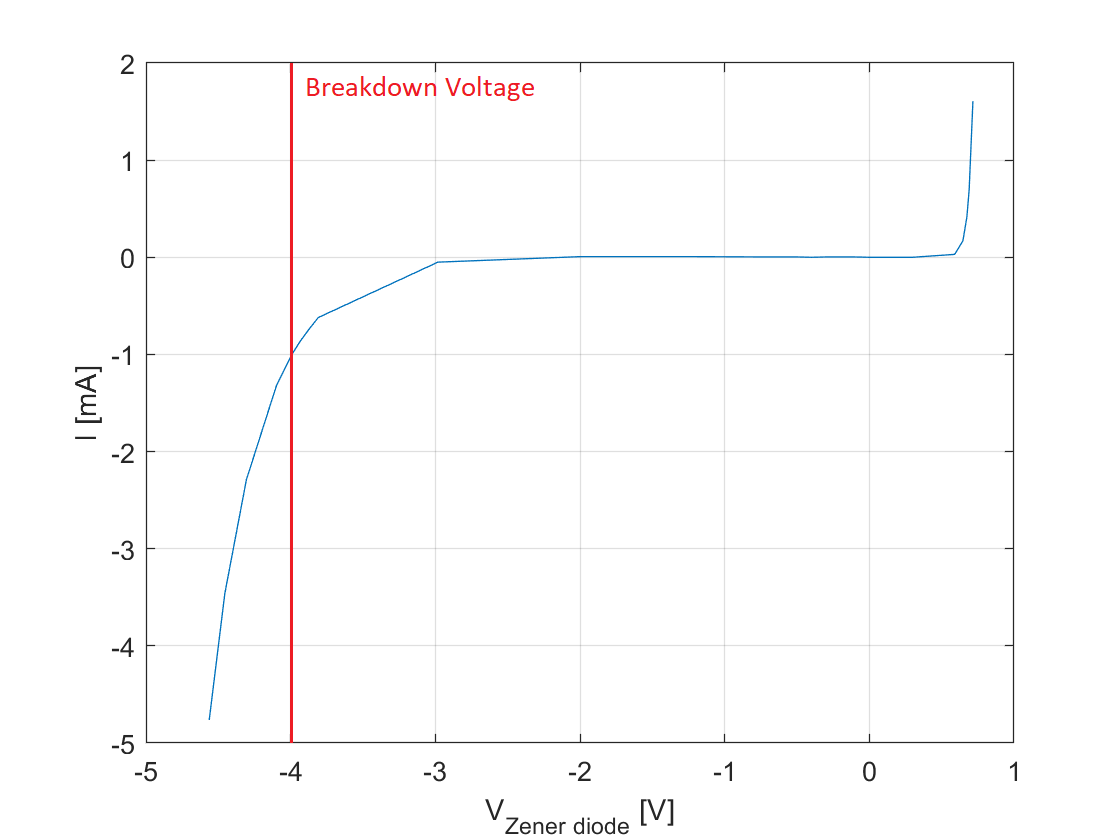
\includegraphics[scale=0.4]{../images/zener_diode.PNG}
	\caption{Measured IV Characteristic Curve of Zener Diode}
	\label{fig:zener_measured}
\end{figure}

\begin{figure}[h!]
	\centering
	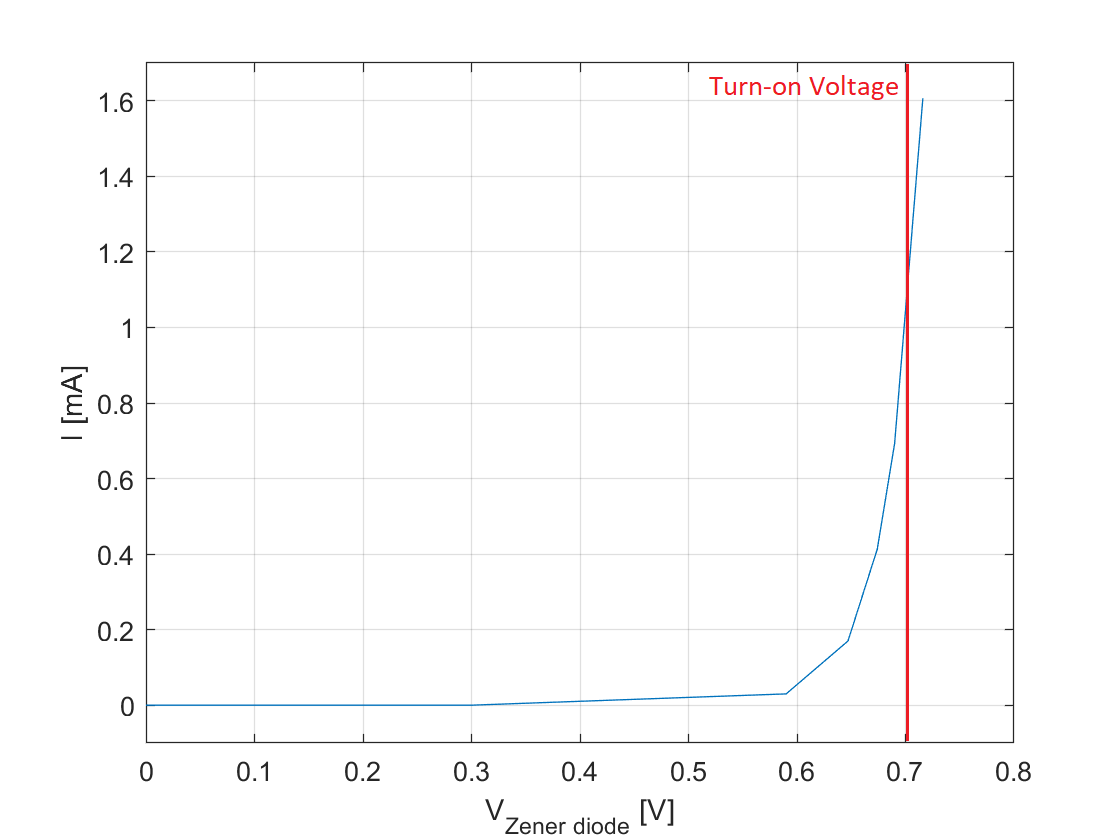
\includegraphics[scale=0.4]{../images/zener_diode_turn_on.PNG}
	\caption{Measured Turn-on Voltage of Zener Diode}
	\label{fig:zener_turn_on}
\end{figure}

\FloatBarrier

Looking more closely at the forward bias portion of the curve (Figure \ref{fig:zener_turn_on}), the turn-on voltage is observed to be approximately $0.7 V$ which is within expectation.

The reverse breakdown voltage of the Zener diode is low enough to be measured in the DC voltage sweep and the value is observed to be approximately $4 V$ (Figure \ref{fig:zener_measured}) which is again a typical value for a Zener diode. Zener diodes are designed to have a low reverse breakdown voltage as they are typically used in the reverse orientation in circuits for the purpose of voltage regulation. (\ref{ref:zener_reg})